\documentclass[a4paper]{article}

\usepackage[margin=2.5cm]{geometry}
\usepackage[pdftex]{graphicx}
\usepackage[utf8]{inputenc}
\usepackage[T1]{fontenc}
\usepackage{textcomp}
\usepackage{babel}
\usepackage{amsmath, amssymb}
\usepackage[colorlinks=true,linkcolor=blue]{hyperref}
\usepackage{float}
\usepackage{mathrsfs}
%\usepackage{enumitem}
%% for identity function 1:
\usepackage{bbm}
%%For category theory diagrams:
%\usepackage{tikz-cd}
%%For code (e.g. python) in latex:
%\usepackage{listings}
%
%Usage: 
%\begin{lstlisting}[language=Python]
%\end{lstlisting}

\newcommand{\incfig}[2][1]{%
\def\svgwidth{#1\columnwidth}
\import{./figures/}{#2.pdf_tex}
}


% figure support
\usepackage{import}
\usepackage{xifthen}
\pdfminorversion=7
\usepackage{pdfpages}
\usepackage{transparent}

\pdfsuppresswarningpagegroup=1

\setlength\parindent{0pt}

\newcommand{\qed}{\tag*{$\blacksquare$}}
\newcommand{\qedwhite}{\hfill \ensuremath{\Box}}

%Inequalities
\newcommand{\cycsum}{\sum_{\mathrm{cyc}}}
\newcommand{\symsum}{\sum_{\mathrm{sym}}}
\newcommand{\cycprod}{\prod_{\mathrm{cyc}}}
\newcommand{\symprod}{\prod_{\mathrm{sym}}}

%Linear Algebra

\DeclareMathOperator{\Span}{span}
\DeclareMathOperator{\Ima}{Im}
\DeclareMathOperator{\diag}{diag}
\DeclareMathOperator{\Ker}{Ker}
\DeclareMathOperator{\ob}{ob}
\DeclareMathOperator{\Hom}{Hom}
\DeclareMathOperator{\sk}{sk}
\DeclareMathOperator{\Vect}{Vect}
\DeclareMathOperator{\Set}{Set}
\DeclareMathOperator{\Group}{Group}
\DeclareMathOperator{\Ring}{Ring}
\DeclareMathOperator{\Ab}{Ab}
\DeclareMathOperator{\Top}{Top}
\DeclareMathOperator{\Htpy}{Htpy}
\DeclareMathOperator{\Cat}{Cat}
\DeclareMathOperator{\CAT}{CAT}
\DeclareMathOperator{\Cone}{Cone}


%Row operations
\newcommand{\elem}[1]{% elementary operations
\xrightarrow{\substack{#1}}%
}

\newcommand{\lelem}[1]{% elementary operations (left alignment)
\xrightarrow{\begin{subarray}{l}#1\end{subarray}}%
}

%SS
\DeclareMathOperator{\supp}{supp}
\DeclareMathOperator{\Var}{Var}

%NT
\DeclareMathOperator{\ord}{ord}

%Alg
\DeclareMathOperator{\Rad}{Rad}
\DeclareMathOperator{\Jac}{Jac}

\DeclareMathAlphabet{\pazocal}{OMS}{zplm}{m}{n}
\newcommand{\unif}{\pazocal{U}}

\begin{document}
    \textbf{1.} Let
    $\sigma_{1,1}  \colon \mathbb{P}^{1} \times \mathbb{P}^{1} \to
    \mathbb{P}^3$ be given by
    \[
    \left[ x_1 : x_2 \right] \times \left[ y_1 : y_2 \right] 
    \mapsto \left[ x_1 y_1 : x_1 y_2 : x_2 y_1 : x_2 y_2 \right] 
    \]  
    (a) It is clear that since
    $(x_1 y_1) (x_2 y_2) - (x_1 y_2) (x_2 y_1) = 0$, 
    $$\sigma_{1,1}\left( \mathbb{P}^{1} \times \mathbb{P}^{1} \right) 
    \subset \mathbb{V} \left( z_1 z_4 - z_2 z_3 \right) 
    = 
    \left\{ \left[ z_1 : z_2 : z_3 : z_4 \right] 
     \colon \text{rank}
 \begin{pmatrix} z_1 & z_2 \\ z_3 & z_4 \end{pmatrix} 
\le 1 \right\}. $$\\
\linebreak
Now, for the converse, suppose 
$z = \left[ z_1 : z_2 : z_3 : z_4 \right] \in 
\mathbb{V} \left( z_1 z_4 - z_2 z_3 \right) $.\\
\linebreak
Then
if $z_1, z_2 = 0$, either $z_3 \neq 0$ or $z_4\neq 0$ (we will omit this from
now), so we have
$\sigma_{1,1}\left( 
\left[ 0 : 1 \right] \times  \left[ z_3 : z_4 \right] \right) 
= \left[ 0 : 0 : z_3 : z_4 \right] =z$.\\
\linebreak
Suppose $z_1, z_3 = 0$, then
$\sigma_{1,1}\left( 
\left[ z_2 : z_4 \right] \times  \left[ 0:1 \right] \right) 
= \left[ 0 : z_2 : 0 : z_4 \right] 
= \left[ z_1 : z_2 : z_3 : z_4 \right] $.\\
\linebreak
If $z_2 , z_4 = 0$ then either $z_1 \neq 0$ or $z_3 \neq 0$ so
$\sigma_{1,1}\left( 
\left[ z_1 : z_3 \right] \times \left[ 1 : 0 \right] \right) = z$.\\
\linebreak
If $z_3, z_4 = 0$ then either $z_1 \neq 0$ or $z_2 \neq 0$, so 
$\sigma_{1,1}\left( 
\left[ 1 : 0 \right]\times \left[ z_1:z_2 \right]  \right) = z$.\\
\linebreak


Suppose $z_1, z_4 = 0$, so either $z_2 \neq 0$ or $z_3 \neq 0$, and in
particular, the other is $0$. Suppose $z_2 = 0$, so $z_3 \neq 0$. Then
$\sigma_{1,1} \left( 
\left[ 0 : z_3 \right] \times \left[ 1 : 0 \right] \right) 
= \left[ 0 : 0 : z_3 : 0 \right] 
= \left[ z_1 : z_2 : z_3 : z_4 \right] $. If instead
$z_3 = 0$, then $z_2 \neq  0$, so
$\sigma_{1,1} \left( \left[ 
z_2 : 0\right] \times \left[ 0 : 1 \right]  \right) 
= \left[ 0 : z_2 : 0 : 0 \right] 
= \left[ z_1 : z_2 : z_3 : z_4 \right] $.\\
If $z_2, z_3 = 0$, then either $z_1$ or $z_4$ is nonzero and the other zero, so
for
$z_1 = 0$,
$\sigma_{1,1} \left( 
\left[ 0 : z_4 \right] \times \left[ 0 : 1 \right]  \right) $ and for
$z_4 = 0$,
$\sigma_{1,1}\left( \left[ z_1 : 0 \right] \times \left[ 1 :0 \right]  \right) 
= z$.\\
\linebreak
Thus we have 
$\mathbb{V} \left( z_1 z_4 - z_2 z_3 \right) 
\subset \sigma_{1,1}\left( \mathbb{P}^{1}\times \mathbb{P}^{1} \right) $.\\
Therefore $\mathbb{V}\left( z_1 z_4 - z_2 z_3 \right) $ is precisely the image
of $\sigma_{1,1}$.\\
\linebreak
(b) Let $\sigma_{1,2}  \colon \mathbb{P}^{1} \times \mathbb{P}^2 \to
\mathbb{P}^{5}$ be the morphism given by
\[
\left[ x_1 : x_2 \right] \times 
\left[ y_1 : y_2 : y_3 \right] 
\mapsto \left[ x_1 y_1 : x_1 y_2 : x_1 y_3 : x_2 y_1 : x_2 y_2 : x_2 y_3
\right] .
\] 
Let $M$ be the matrix
\[
    M = \begin{pmatrix} z_1 & z_2 & z_3\\
    z_4 & z_5 & z_6 \end{pmatrix} 
\] 
We claim that
 \[
\sigma_{1,2} \left( \mathbb{P}^{1} \times \mathbb{P}^{2} \right) 
= \left\{ 
\left[ z_1 : \ldots : z_6 \right]  \mid 
\text{rank}M \le 1 \right\} = A
\] 
This is equivalent to showing that
$\sigma_{1,2}\left( \mathbb{P}^{1}\times \mathbb{P}^2 \right) $ is the
vanishing
of the  $2 \times 2$ minors of $M$.\\
\linebreak
Now, since $z_1 z_5 - z_4 z_2 = x_1 y_1 x_2 y_2
- x_2 y_1 x_1 y_2 = 0$ and
$z_2 z_6 - z_5 z_3 = x_1 y_2 x_2 y_3 - x_2 y_2 x_1 y_3 = 0$, we have that
$\sigma_{1,2}\left( \mathbb{P}^{1}\times \mathbb{P}^2 \right) 
\subset A   $.\\
\linebreak
Now, suppose conversely, that
$z = \left[ z_1 : \ldots : z_6 \right] 
\in A$, so
$z_1 z_5 - z_4 z_2 = 0 = z_2 z_6 - z_5 z_3$.\\
\linebreak
If $z_1 = z_2 = z_3 = 0$ then
$\sigma_{1,2}\left( 
\left[ 0 : 1 \right]
\times \left[ z_4 : z_5 : z_6 \right]   \right) 
= z $ (here $z_4, z_5 $ and $z_6$ cannot all be $0$ as
$\left[ 0: \ldots : 0 \right] \not\in \mathbb{P}^{5}$ ).
If $z_i \neq 0$ for some $i \in \left\{ 1,2,3 \right\} $, then 
$z_{i+3} z_1 = z_i z_4$, since for $i = 1$, we get
$z_1 z_4 = z_1 z_4$, for $i=2$ we get
$z_1 z_5 = z_2 z_4$ which is true since
 $z \in A$ and $\begin{pmatrix} z_1 & z_2\\ z_4 & z_5 \end{pmatrix} $ is a 
 $2\times 2$ minor of $M$; if
 $i= 3$, we get $z_1 z_6 = z_3 z_4$ which is true as
 $\begin{pmatrix} z_1 & z_3 \\ z_4 & z_6 \end{pmatrix} $ is a 
 $2\times 2$ minor of $M$.\\
 Completely equivalently, one can show that
 $z_{i+3} z_2 = z_i z_5$ and $z_{i+3} z_3 = z_i z_6$ which follow
 from the $2\times 2$ minors in $M$.\\
 Thus
 \begin{align*}
\sigma_{1,2}
\left( \left[ z_i : z_{i+3}  \right] \times 
\left[ z_1 : z_2 : z_3 \right] \right)
&= 
\left[ z_i z_1 : z_i z_2 : z_i z_3 : z_{i+3} z_1 : z_{i+3} z_2 : z_{i+3} z_3
\right] \\
&=\left[ z_i z_1 : z_i z_2 : z_i z_3 : z_i z_4 : z_i z_5 : z_i z_6 \right] \\
&= \left[ z_1 : z_2 : z_3 : z_4 : z_5 : z_6 \right] 
= z 
 \end{align*}

 (c) This generalizes directly to letting $M$ be the matrix
 $M = (z_{ij})$ with $z_{ij} = x_i y_j$ and
 $k = 1$.\\
 \linebreak
 \textbf{2:}\\
 (a) Let $\varphi  \colon k\left( \mathbb{P}^{1} \right) 
 \to k(x)$ be defined by
 $\frac{F}{G} \mapsto \frac{F(x,1)}{G(x,1)}$.\\
 One-to-one: By definition of being fields, we have
 $\frac{F}{G}+ \frac{F'}{G'} = \frac{FG' + F'G}{G G'}$, so
 $\varphi \left( \frac{F}{G}+ \frac{F'}{G'} \right) 
 = \frac{F(x,1) G'(x,1) + F'(x,1) G(x,1)}{G(x,1)G'(x,1)}
 = \frac{F(x,1)}{G(x,1)} + \frac{F'(x,1)}{G'(x,1)}
 = \varphi\left( \frac{F}{G} \right) 
 + \varphi \left( \frac{F'}{G'} \right) $, so
 $\varphi$ is a homomorphism.\\
 It suffices to show that
 $\varphi \left( \frac{F}{G} \right) = 0 \implies
 \frac{F}{G}=0$.\\
 First, $\Gamma_h (\mathbb{P}^{1})
 = \frac{k\left[ x,y \right] }{\mathbb{I} \left( \mathbb{P}^{1} \right) }
 = k\left[ x,y \right] $, so
 $F,G \in k\left[ x,y \right] $ are forms of the same degree with
 $G \neq 0$.\\
 Suppose $\varphi \left( \frac{F}{G} \right) = \frac{F(x,1)}{
 G(x,1)}=0$. Then
 $F(x,y) \in (y-1)$. We claim
 $F = 0$:\\
 Suppose $F(x,y) = \left( g_0 + g_1+ \ldots + g_m \right) 
 (y-1)$ with $g_m \neq 0$. Then
 $F_{m+1} = g_m z \neq 0$, so all lower $F_i$ vanish as
 $F$ is homogeneous. So $0 = F_0 = -g_0$. Then
 $0 = F_1 = g_0 z - g_1 \implies g_1 = 0$. Assume
 $g_0 , \ldots, g_j = 0$, then
 $0 = F_{j+1}
 = g_{j} z - g_{j+1} = - g_{j+1}$, so
 $g_{j+1} = 0$. Hence
 $g_0, \ldots, g_m = 0$, contradicting
 $g_m \neq 0$. Thus
 $g = g_0 + \ldots + g_m = 0$ implying $F = 0$.\\
 Thus 
 $G \in k - \left\{ 0 \right\} $, so
 $\frac{F}{G} = 0$.\\
 Onto: Now suppose $\frac{f}{g} \in k(x)$, so $g \neq 0$.
 Let $d = \max \left\{ \deg f , \deg g \right\} $, and
 let  $f' = H_d(f)$ and $g' = H_d(g)$ be the homogenizations of
 $f$ and $g$ of degree $d$ in
 $k\left[ x,y \right] $. Then
 $f' (x,1) = f$ and $g' (x,1) = g$ and
 $f',g'$ are forms of degree
 $d$ with
 $g' \neq 0$. Then
 $\varphi \left( \frac{f'}{g'} \right) 
 = \frac{f'(x,1)}{g'(x,1)}= \frac{f(x)}{g(x)}$, so
 $\varphi$ is onto.\\
 \linebreak
 (b) We have that $\varphi  \colon X \to Y$ is dominant if
 $\mathbb{I} \left( \varphi (X) \right) = \mathbb{I}(Y)$
 if and only if $
 \mathbb{V} \left( \mathbb{I} \left( \varphi(X) \right)  \right) 
 = \mathbb{V} \left( \mathbb{I}\left( Y \right)  \right) 
 = Y$.\\
 Now, $\varphi(X) \subset \mathbb{V}\left( \mathbb{I}\left( Y \right)  \right)
 $, and supposing $W$ is a projective algebraic set containing
 $\varphi(X)$, we have
 $\mathbb{I}(Y) = \mathbb{I}\left( \varphi(X) \right) \supset
 \mathbb{I}(W)$, so
 $\mathbb{V}\left( \mathbb{I}\left( 
 \varphi(X) \right)  \right) =  \mathbb{V} \left( \mathbb{I}(Y) \right) 
 \subset  \mathbb{V}\left( \mathbb{I}\left( W \right)  \right) 
 = W$, so $\mathbb{V} \left( \mathbb{I}\left( \varphi(X) \right)  \right) $ 
 is the smallest projective algebraic set containing
 $\varphi(X)$. Hence
 $\mathbb{V} \left( \mathbb{I}\left( \varphi(X) \right)  \right) 
 = \overline{\varphi(X)}$
 , so we see that the equivalence
 $\varphi$ dominant if and only if
 $\overline{\varphi (X)} = Y$ is also true for the projective case.
 Now $\overline{\varphi(X)}- U =  Y - U$ is closed,
 so $\varphi^{-1}
 \left( \overline{\varphi(X)}- U \right) 
= \varphi^{-1} \left( \overline{\varphi(X)} \right) 
 - \varphi^{-1}(U)
 = X - \varphi^{-1}(U)$ is closed, so
 $\varphi^{-1}(U)$ is open.\\
 \linebreak
 \textbf{3:}\\
 (a) By the lemma on lecture note 24, we have that since
 $\varphi  \colon X \to Y$ is an isomorphism
 with $X \subset \mathbb{P}^{n}$ and
 $Y \subset \mathbb{P}^{m}$, the pullback
 $\varphi^{*}  \colon k(Y) \to k(X)$ is an isomorphism.\\
 Suppose $\psi  \colon Y \to X$ is the inverse to $\varphi$. By the lemma on
 lecture note 24, we have that  $\psi^{*}$ is the inverse to $\varphi^{*}$.\\
 It thus remains to show that $\varphi^{*}$ takes 
 $\mathcal{O}_Q (Y)$ into $\mathcal{O}_P(X)$, that
 $\psi^{*}$ takes $\mathcal{O}_P(X)$ into $\mathcal{O}_Q(Y)$ and
  that $\psi^{*} \circ \varphi^{*}$ is the identity on
  $\mathcal{O}_Q(Y)$ and that
  $\varphi^{*} \circ \psi^{*}$ is the identity on $\mathcal{O}_P(X)$.\\
  \linebreak
 Suppose $\left( U, \alpha \right) \in 
 \mathcal{O}_Q(Y)$. That is, $Q \in U$. Now, $P \in X$ and
 $\varphi$ is a morphism, so we can find some open set
 $W$ containing $P$ such that $\varphi|_W$ agrees with some map
 $U \to \mathbb{P}^{m}$ with
 $A \mapsto  \left[ F_1 (A) : \ldots : F_{m+1}(A) \right] $ for
 $F_1, \ldots, F_{m+1}$ homogeneous of the same degree.
 Thus $P \in \varphi^{-1}(Y) \cap W := U'$, and thus
 $\varphi^{*} \left( U, \alpha \right) 
 = \left( U', \alpha \circ \varphi \right) \in \mathcal{O}_P(X) $ since
 if $\alpha = \frac{G}{H}$, then
 $\left( \alpha \circ \varphi \right) (P)
 = \frac{G \left( F_1(P), \ldots, F_{m+1}(P) \right) }{
 H \left( F_1(P), \ldots, F_{m+1}(P) \right) }
 = \frac{G(Q)}{H(Q)}$ is well defined.\\
 Since $\psi (Q) = P$, we can repeat the above to find that
 $\psi^{*}$ maps $\mathcal{O}_P(X)$ into $\mathcal{O}_Q(Y)$. Now, we further
 have
 that for any $(U, \alpha) \in \mathcal{O}_Q(Y)$,
 $\psi^{*} \circ \varphi^{*} \left( U, \alpha \right) 
 = \psi^{*} \left( U', \alpha \circ \varphi \right) 
 = \left( U'', \alpha \circ \varphi \circ \psi \right) 
 = \left( U'', \alpha \right) = (U, \alpha) $, and similarly,
 for any  $(U, \alpha) \in \mathcal{O}_P(X)$, 
 $\varphi^{*} \circ \psi^{*}\left( U, \alpha \right) 
 = \varphi^{*} \left( U', \alpha \circ \psi \right) 
 = \left( U'', \alpha \circ \varphi \circ \varphi \right) 
 = (U'', \alpha) = (U, \alpha)$, so we can thus conclude that $\varphi^{*}$ 
 restricts to an isomorphism
 $\varphi^{*}|_{\mathcal{O}_Q(Y)}  \colon
 \mathcal{O}_Q(Y) \to \mathcal{O}_P(X)$.\\
It remains to show that this is a homomorphism of rings.\\
Suppose $(U, \alpha), (V, \beta) \in \mathcal{O}_Q(Y)$. Then
indeed $(U,\alpha) + (V,\beta) = \left( U \cap V, \alpha|_{U \cap V}
+ \beta|_{U \cap V} \right) \in 
\mathcal{O}_Q(Y)$ and
$\left( U, \alpha \right) \cdot  \left( V, \beta \right) 
= \left( U \cap V \right) , 
\alpha|_{U \cap V} \cdot \beta|_{U \cap V})
\in \mathcal{O}_Q(Y)$ since
$Q \in U \cap V$.\\
Now 
\begin{align*}
\varphi^{*}
\left( \left( U \cap V , \alpha|_{U \cap V}+ \beta|_{U \cap V} \right)  \right) 
&= \left( W \cap \varphi^{-1}(U) \cap \varphi^{-1}(V), \alpha|_{U \cap V}\circ \varphi + 
\beta|_{U \cap V} \circ \varphi\right)\\
&= 
\left( W \cap \varphi^{-1}(U), \alpha|_{U\cap V}\circ \varphi \right) 
+ \left( W \cap \varphi^{-1}\left( V \right) ,
\beta|_{U \cap V} \circ \varphi \right) 
= \varphi^{*} \left( U , \alpha \right) 
+ \varphi^{*} \left( V, \beta \right).
\end{align*}
And replacing the $+$ with $\cdot $, we get
$\varphi^{*} \left( \left( U, \alpha \right) \cdot 
\left( V, \alpha \right) \right) 
= \varphi^{*} \left( U,\alpha \right) \cdot 
\varphi^{*} \left( V, \beta \right) $ also.\\
Hence $\varphi^{*}$ is a ring homomorphism.\\
\linebreak



 We recall that 
 \[
 m_P(X) = \left\{ f \in \mathcal{O}_P(X)  \colon f(P)=0 \right\} 
 = \left\{ \text{non-units in } \mathcal{O}_P(X) \right\}
 = \left\{ (U, \alpha)  \colon P \in U, \alpha(P)=0 \right\} 
 \] 
 
 Now, suppose $(U, \alpha) \in m_Q(Y)$. Then
 $\varphi^{*} \left( U, \alpha \right) 
 = (U', \alpha \circ \varphi)$ where $P \in U'$ and
 since $\alpha \circ \varphi (P) = \alpha (Q) = 0$, we have
 $(U', \alpha \circ \varphi) \in m_P(X)$. Similarly, we get
 $\psi^{*} (U, \alpha) \in m_Q(Y)$ for any
 $(U,\alpha) \in m_P(X)$.\\
 Showing that
 $\psi^{*} \circ \varphi^{*} \left( U, \alpha \right) = (U, \alpha)$ for any
 $(U, \alpha) \in m_Q(Y)$ and
 $\varphi^{*} \circ \psi^{*} \left( V, \beta \right) =
 (V, \beta)$ for any $(V, \beta) \in m_P(X)$ is done the same as the first part
 of the problem. Thus
 $\varphi^{*}|_{\mathcal{O}_Q(Y)}$ restrict to an isomorphism
 $\varphi^{*}|_{m_Q(Y)} \colon m_Q(Y) \to m_P(X)$. It remains to show that this
 isomorphism is, in fact, a homomorphism. It suffices to show this for
 $\varphi^{*}$.\\
 Letting $\left( U, \alpha \right) , \left( V, \beta \right) 
 \in m_Q(Y)$, we have $Q \in U \cap V$ and $\alpha(Q) = 0 = \beta(Q)$. Thus
 since $(U, \alpha) + \left( V, \beta \right) 
 = \left( U \cap V, \alpha + \beta \right) $, we get
 \begin{align*}
 \varphi^{*} \left( (U, \alpha) + (V, \beta) \right) 
 = \varphi^{*} \left( U \cap V, \alpha + \beta \right) 
 &= \left( W \cap \varphi^{-1}(U) \cap \varphi^{-1}(V),
 \alpha \circ \varphi + \beta \circ \varphi \right)\\
 &= (W \cap \varphi^{-1}(U), \alpha \circ \varphi) + 
 (W \cap \varphi^{-1}(V), \beta \circ \varphi)
 = \varphi^{*}\left( U,\alpha \right) 
 + \varphi^{*}\left( V, \beta \right),
 \end{align*}
 showing that $\varphi^{*}$ is an isomorphism of abelian groups.\\
 \linebreak
 (b) Suppose $\varphi  \colon X \to Y$ is an isomorphism. By (a), we have
 that $\varphi^{*}$ restricts to an isomorphism of abelian groups
 $m_Q(Y) \to m_P(X)$.\\
 We thus have that $\frac{m_P(X)}{m_P(X)^2}$ which is a quotient group is
 isomorphic to $\frac{m_Q(Y)}{m_Q(Y)^2}$, and hence, if $X$ is smooth, then
 \[
     \dim Y = \dim X \stackrel{\text{X smooth}}{=}
     \dim_k \frac{m_P(X)}{m_P(X)^2}
     = \dim_k \frac{m_Q(Y)}{m_Q(Y)^2}
 \] 
 so $Y$ is smooth. If $Y$ were smooth instead, interchange $X$ and $Y$ above,
 as well as $P$ and $Q$, giving that $X$ is smooth as well. So
 $X$ is smooth if and only if $Y$ is smooth.\\
 \linebreak
 (c) We have that
 $\Gamma \left( V(y) \right) 
 = k\left[ x,y \right] / I(V(y)) 
 = k\left[ x,y \right] / \sqrt{(y)} 
 = k\left[ x,y \right] / (y)
 = k\left[ x \right] $ and
 $\Gamma\left( V(y-x^3) \right) 
 = k\left[ x,y \right] / I \left( V\left( y-x^3 \right)  \right) 
 = k\left[ x,y \right] / \sqrt{(y-x^3)} 
 = k\left[ x,y \right] / \left( y-x^3 \right) 
 = k\left[ x \right] $, and
 $k\left[ x \right] \cong k\left[ x \right] $ by the trivial isomorphism (here
 we have concluded that the $\sqrt{(y)} = (y)$ and
 $\sqrt{(y-x^3)}  = (y-x^3)$ since it is given in the problem that
 $V(y)$ and $V(y-x^3)$ are varieties. Thus
 $\Gamma(V(y)) \cong \Gamma\left( V(y-x^3) \right) $, so by the lemma
 on page 2 of lecture note 8, we have that
 $V(y)$ and $V(y-x^3)$ are isomorphic as affine algebraic varieties.\\
 \linebreak
 (d) The projective closure of a set $X \subset \mathbb{A}^{n}$ in
 $\mathbb{P}^{n}$ is $\mathbb{V}\left( H\left( I(X) \right)  \right) $ by
 a lemma on lecture note 19.
 Thus, the projective closure of $V\left( y-x^3 \right) $ is
 $\mathbb{V}\left( H \left( I\left( V(y-x^3) \right)  \right)  \right) 
 \stackrel{\text{variety}}{=} \mathbb{V}(H(y-x^3))
 \stackrel{\text{principal ideal}}{=}
 \mathbb{V}\left( yz^2 - x^3 \right) $, since homogenizing a principal ideal is
 homoginizing the generator. Now, if $P \in \mathbb{V}(y)$, then
 $P = \left[ a: 0 : b \right] $, so
 $P \not\in U_2$. Suppose $P \in U_1$, then
 since $\mathbb{V}(y) \cap U_1 = V(y)$ and
 $\frac{d}{dy} y = 1 \neq 0$, we have that $P$ is not a singular point
 of $\mathbb{V}(y)$. Similarly, if $P \in U_3$, then
 $\mathbb{V}(y) \cap U_3 = V(y)$ and
 $\frac{d}{dy} y = 1 \neq 0$ again, so $P$ is not a singular point of
 $\mathbb{V}(y)$. Hence $P$ is smooth by definition.\\
 By (b), if $\mathbb{V}(y)$ and $\mathbb{V}(yz^2 - x^3)$ were isomorphic, then
 $\mathbb{V}(yz^2 - x^3)$ would be smooth as well. However, we have
 $\left[ 0 : 1 : 0 \right] \in \mathbb{V}(yz^2 - x^3), U_2$, so
 $\mathbb{V}\left( yz^2 - x^3 \right) \cap U_2
 = V(z^2 - x^3)$, and letting $f = z^2 - x^3$, we have
 $f_x = -3x^2$ and $f_z = 2z$, so
 evaluating at $(0,0)$, we have
 $f_x (0,0) = 0 = f_z (0,0)$, so
 $\mathbb{V}(yz^2 - x^3)$ is singular at $\left[ 0:1:0 \right] $. Thus
 the projective closures of $V(y)$ and $V(y -x^3)$ are not isomorphic.\\
 Geometrically, we see that $\mathbb{V}(yz^2 - x^3) \cap 
 U_2 = V(z^2 - x^3)$ has a cusp at $(0,0)$ making it not smooth here while
 $\mathbb{V}(y) \cap U_2$ is the single point.

 \begin{figure}[H]
     \centering
     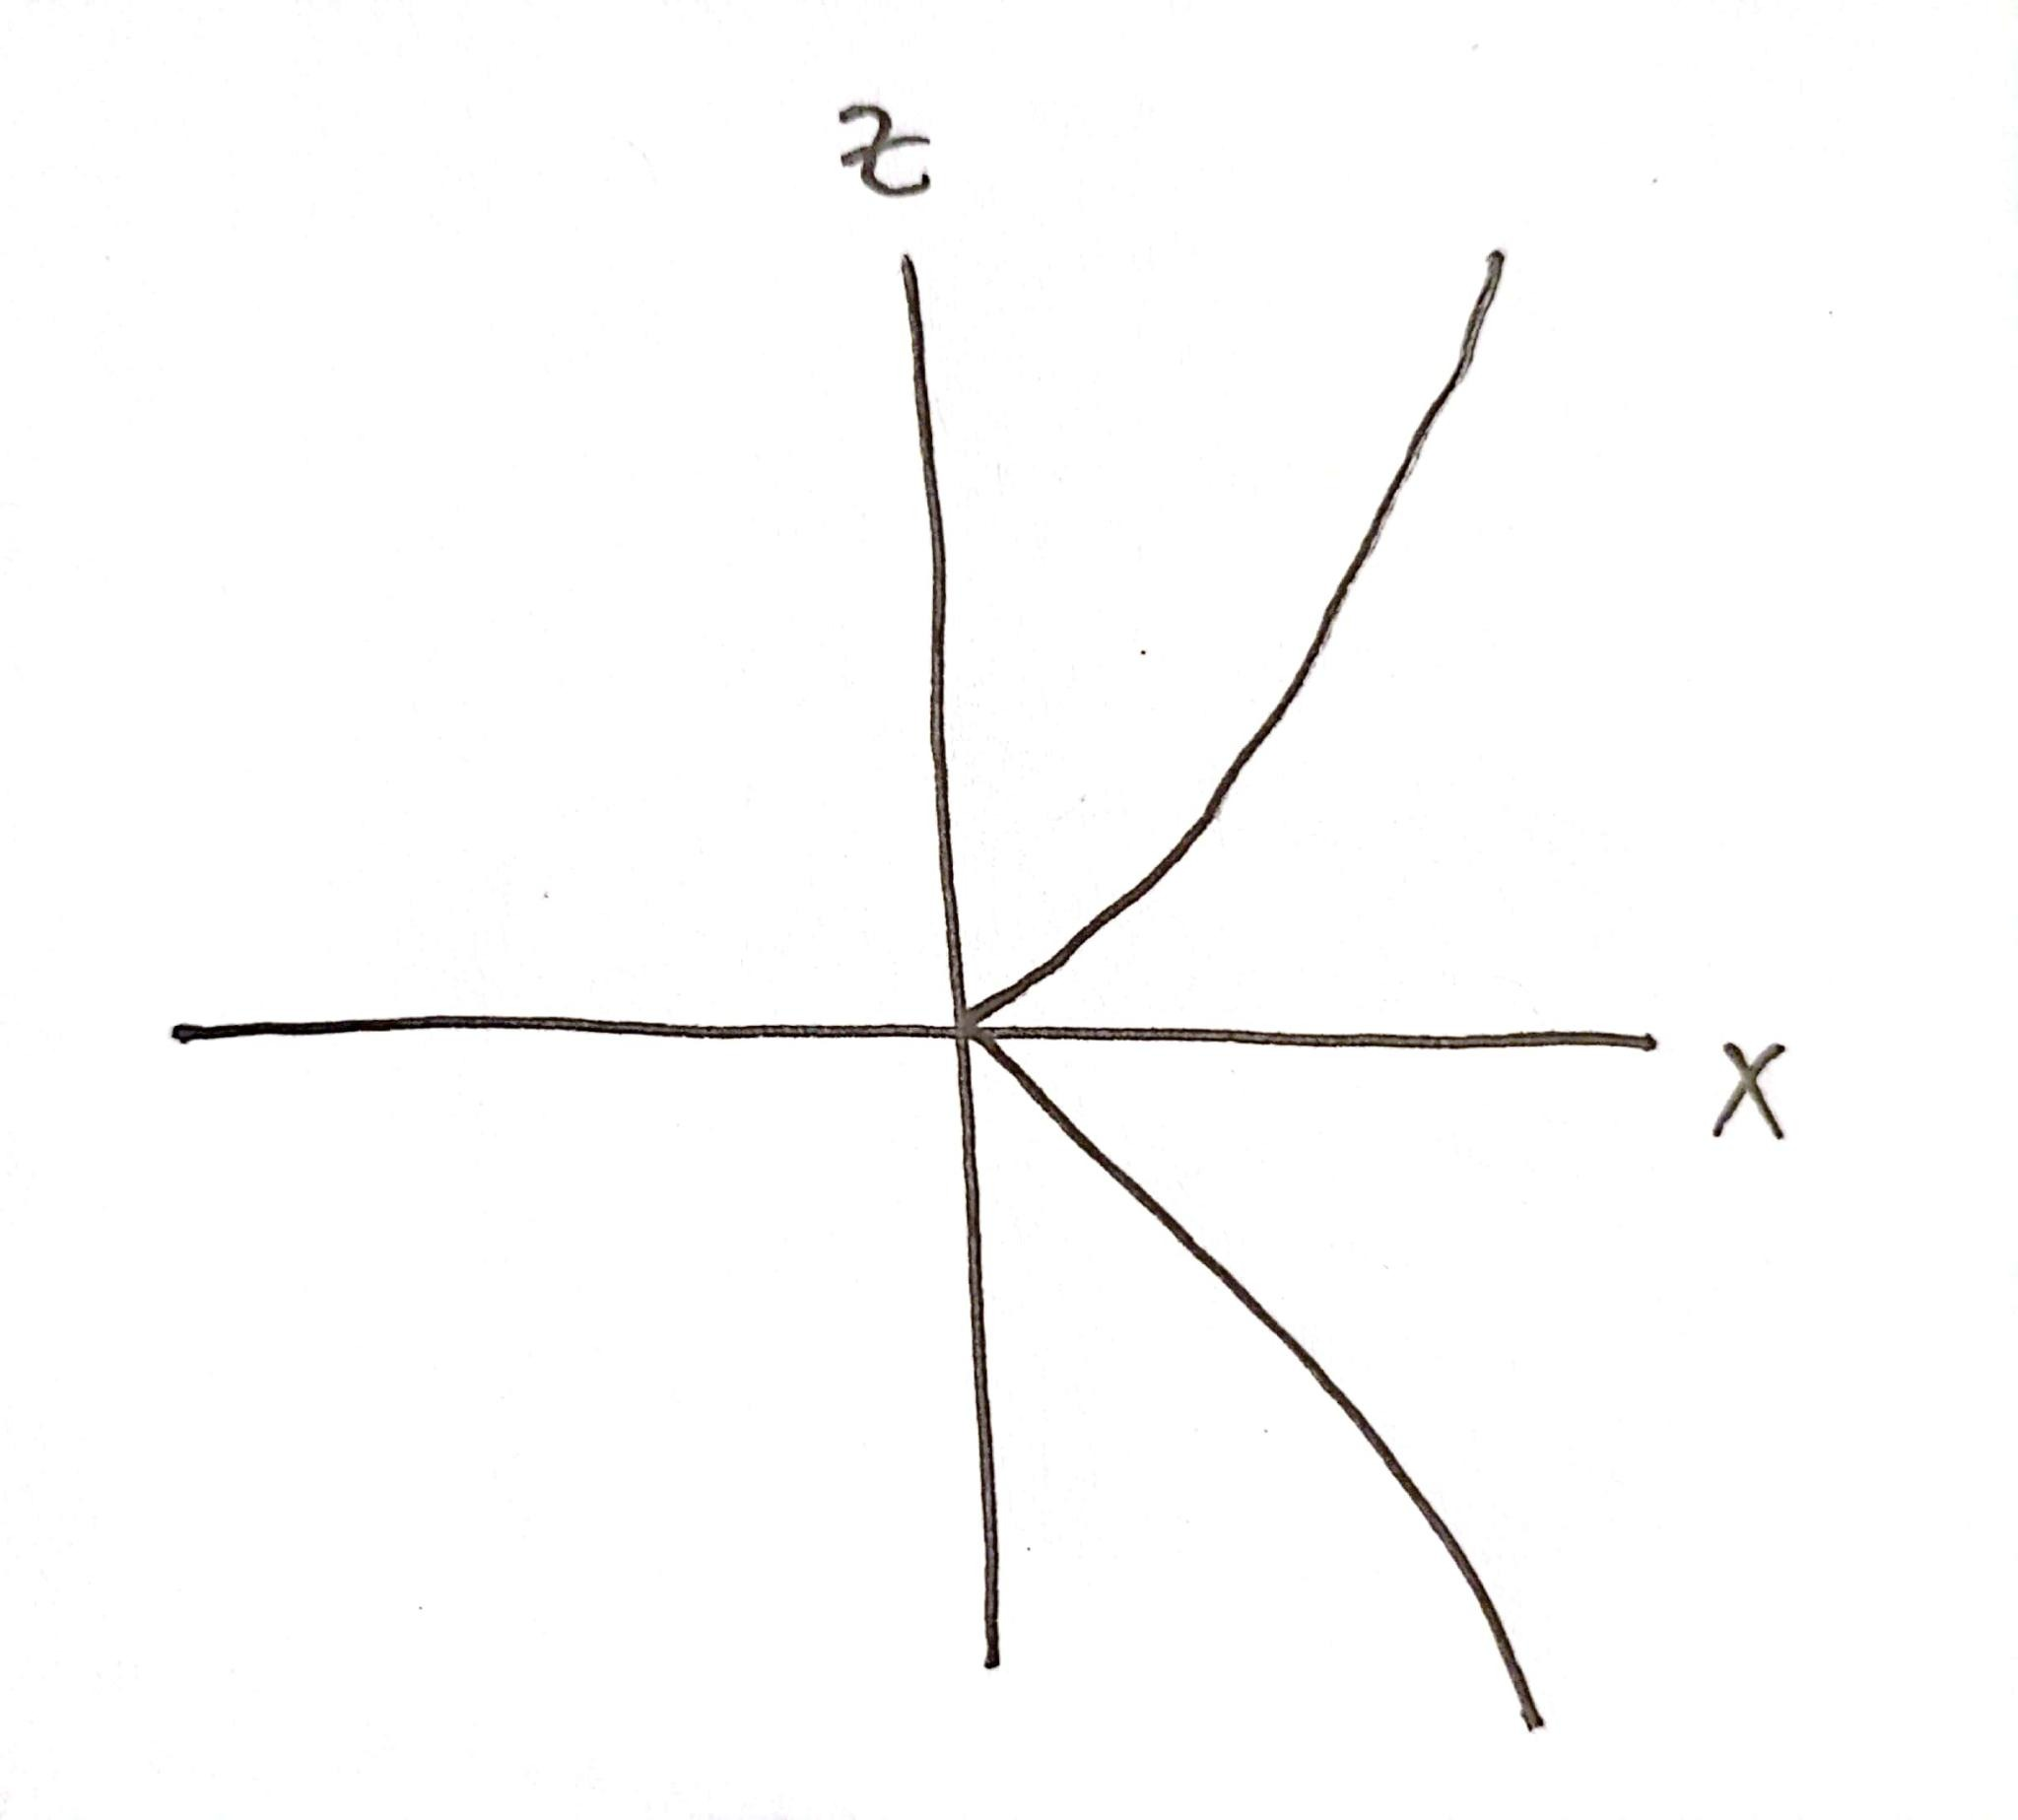
\includegraphics[width=0.5\textwidth]{3d.jpeg}
     \label{fig:3d-jpeg}
 \end{figure}

 \textbf{4:}\\
 Let $F \in k\left[ x,y,z \right] $ be a homogeneous polynomial of degree
 $n$.\\ 
 (a) We can write
 \[
     F = \sum_{i+j+k = n, i,j,k\ge 0} \alpha_{i,j,k} x^{i}y^{j}z^{k}.
 \] 
 Then 
 \begin{align*}
     F_x &= \sum_{i+j+k=n, i\ge 1} \alpha_{i,j,k}\cdot i x^{i-1}y^{j}z^{k}\\
     F_y &= \sum_{i+j+k=n, j\ge 1} \alpha_{i,j,k}\cdot j x^{i}y^{j-1}z^{k}\\
     F_z &= \sum_{i+j+k=n, k\ge 1} \alpha_{i,j,k}\cdot k x^{i}y^{j}z^{k-1}
 \end{align*}
 so
 \begin{align*}
     x F_x &= \sum_{i+j+k=n, i\ge 1} \alpha_{i,j,k}\cdot i x^{i}y^{j}z^{k}\\
     yF_y &= \sum_{i+j+k=n, j\ge 1} \alpha_{i,j,k}\cdot j x^{i}y^{j}z^{k}\\
     yF_z &= \sum_{i+j+k=n, k\ge 1} \alpha_{i,j,k}\cdot k x^{i}y^{j}z^{k}.
 \end{align*}
giving the sum
\begin{align*}
    xF_x + y F_y + z F_z = \sum_{i+j+k = n, i,j,k\ge 0}
    a_{i,j,k} (i+j+k) x^{i} y^{j} z^{k}
    = n F.
\end{align*}

(b) 
\textit{Claim:} $f_x = D(F_x)$.\\
\textit{Proof:} Suppose $F = \sum_{i+j+k = n}
\alpha_{i,j,k} x^{i}y^{j}z^{k}$. Then
$F_x = \sum_{i+j+k = n, i \ge 1} \alpha_{i,j,k}i x^{i-1}y^{j}z^{k}$. So
$D(F_x) = \sum_{i+j+k = n, i\ge 1} \alpha_{i,j,k}i x^{i-1}y^{j}$.\\
Now $f = \sum_{i+j+k = n} \alpha_{i,j,k} x^{i}y^{j}$, so
$f_x = \sum_{i+j+k = n, i \ge 1} \alpha_{i,j,k} i x^{i-1}y^{j}$, proving the
claim.\\
\linebreak

Suppose that $P$ is a singular point of $\mathbb{V}(F)$ with
$P \in U_3$. Thus $P$ is a singular point of $V(F(x,y,1)) = V(f)$ which means
that $f_x (P) = 0 = f_y(P)$ and $f(P) = 0$. But if we denote the dehomoginization operator by
$D$, we get that $f_x = D\left( F_x \right) $, so
$D\left( F_x \right) (P) = 0 = D(F_y)(P)$. Further, $P \in V
(F(x,y,1))$ gives that $F(P) = 0$. Now,
$z(P) F_z(P) = n F(P) = 0$ so since $P \in U_3, F_z(P)=0$. Similarly for if
$P \in U_2$ or $U_1$.\\
Conversely, if $F(P) = F_x(P) = F_y(P) = F_z(P) = 0$ then suppose $P \in U_3$
wlog, with $P = \left[ a, b, 1 \right] $. Note that
$F_i$ is homogenous for $i = x,y,z$. Then $f_x (P) = D(F_x)(a,b,1)  
= F_x(a,b,1) = 0 $. And similarly $f_y (P) = 0$. And
$f(P) = D(F)(a,b,1) = F(a,b,1) = 0$ since $F$ is homogeneous.
Thus
$P$ is a singular point of $\mathbb{V}(F)$.\\
\linebreak
(c) 



















\newpage




\textbf{5:} \\
(a) Let $F = x^2 y^3 + x^2 z^3 + y^2 z^3$. Let $X = \mathbb{V} (F)$. Then by
problem 4.(b), we have that $P$ is a singular point if and only if
$F(P) = F_x(P) = F_y(P) = F_z(P) = 0$. Now
$F_x = 2xy^3 + 2xz^3$, $F_y = 3x^2 y^2 + 2yz^3$ and
$F_z = 3x^2 z^2 + 3y^2 z^2 = 3 z^2 \left( x^2 + y^2 \right) $. If
$z = 0$ then $x^2 y^2 = 0$ so either $x = 0$ or $y = 0$.\\
\linebreak
If $x = 0$ then $y z^3 = 0$, so either $y =0$ or $z = 0$. If
$y = 0$ then $x =0$ or $z=0$.\\
If none of them are $0$, then 
$x^2 = -y^2$ and $y^3 = -z^3$ and $-2z^3 = 3 x^2 y$. However, 
from the first two, we get $3x^2 y = 3z^3$, so $-2z^3 = 3z^3$, hence
$5 z^3 = 0$ so $z = 0$, contradiction.\\
So the only singular points are 
$\left\{ \left[ 1:0 :0 \right] , \left[ 0 : 1 : 0 \right] ,
\left[ 0 : 0 : 1 \right] \right\} $.\\
\linebreak
Let $f = F(x,y,1) = x^2 y^3 + x^2 + y^2 $, so
the multiplicity at $(0,0)$ is $2$, and the tangent cone is
$V(x^2 + y^2))$.\\
\linebreak
Let  $f = F(x,1,z) = x^2 + x^2 z^3 + z^3$, so the multiplicity at $(0,0)$ is
$2$, and the tangent cone at $(0,0)$ is $V(x^2)$.\\
\linebreak
Let $f = F(1,x,z) = y^3 + z^3 + y^2 z^3$, so multiplicity at $(0,0)$ is $3$ and
the tangent cone is $V\left( y^3 + z^3 \right) $.\\
\linebreak
(b) Let $F = y^2 z - x ( x-z) ( x-\lambda z), \lambda \in k$. Then
$F_x = - (x-z) ( x- \lambda z) - x (x- \lambda z) - x (x-z)$, and
$F_y = 2yz$ and  $F_z = y^2 + x (x- \lambda z) + \lambda x (x-z)$. 
If $y = 0$ then 
$x \left( x- \lambda z + \lambda x - \lambda z \right) $. If $x = 0$ then
$z \neq 0$ and $\lambda = 0$. If $x \neq 0$ then
$x (1+\lambda ) = 2 \lambda z$. Also $x = z$ or
$x = \lambda z$, so
$ \frac{2 \lambda}{1+\lambda} \in \left\{ 1, \lambda \right\} $, so
either $\lambda = 1$ or $\lambda^2 = \lambda \implies \lambda \in \left\{ 0,1
\right\} $. Or $\lambda = -1$ in which case $z = 0$ we get
$\left[ 1 : 0 : 0 \right] $, in either case $x = z$, but inserting into $F_x$,
we get
$\lambda = 1$.\\
Now, if $z = 0$ then $x = 0$ so $y \neq 0$.\\
So all the singular points are 
\[
\left\{ \left[ 0 : 0 : 1 \right] ,
\left[ 1 : 0 : 1 \right] ,
\left[ 0 : 1 : 0 \right]  \right\} 
\] 
Let $f = y^2 - x^2 (x-z)$, then the multiplicity of $(0,0)$ is
$2$ and tangent cone $V(y^2)$.\\
For $f = y^2 - x (x-1)^2$ for $(0,1)$, we insert  $x'+1$, so
 $y^2 - (x'+1) x'^2$ which has multiplicity $2$ and
 cone $V\left( y^2 - x'^2 \right) $ which maps to
 $V \left( y^2 - (x-1)^2 \right) $.\\
 \linebreak
 Let $f = z - x (x-z) (x- \lambda z)$ which has multiplicity $1$ and
 cone $V(z)$.\\
 \linebreak
\textbf{6:}\\
(a) Firstly, $v_{2,2}(P) =
\left[ x_0^2 : x_0y_0 : x_0 z_0 : y_0^2 : y_0 z_0 : z_0^2 \right] $, so
$v_{2,2}(P)^{*} = \mathbb{V}\left( x_0^2 w_1+ x_0 y_0 w_2+ \ldots y_0z_0 w_5 +
 z_0^2 w_6 \right) $.\\
 \linebreak
 If $P \in C$ with $\left[ C \right] =
 \left[ a : b : c : d : e : f \right] $, then
\[
 a x_0^2 + b x_0 y_0 + c x_0 z_0 + dy_0^2 + ey_0 z_0 +
f z_0^2 = 0
\]
so $\left[ C \right] \in v_{2,2}(P)^{*}$. Conversely, for any
$\left[ C \right] \in v_{2,2}(P)^{*}$, we have
$P \in C$ by the nature of $v_{2,2}$.\\
\linebreak
(b) We have that $P_1, \ldots, P_5 \in C$ if and only if
$v_{2,2}(P_1)^{*} \cap \ldots \cap v_{2,2}(P_5)^{*}$ is nonempty, which is true
by problem 4 on homework 10.\\
\linebreak
(c) Suppose $P = \left[ 0:0:1 \right] $. Then











\newpage
Let $f$ be the homogenization of
$F$ with respect to $z$, so
 \[
f = \sum_{i+j+k = n, i,j,k\ge 0} \alpha_{i,j,k}x^{i}y^{j}
\] 
Then $f_x = \sum_{i+j+k =n, i\ge 1} \alpha_{i,j,k} i x^{i-1}y^{j}$ and
$f_y = \sum_{i+j+k = n, j\ge 1} \alpha_{i,j,k}j x^{i}y^{j-1}$ vanish at
$P$.\\
\linebreak
(c) 
 







\end{document}
